\chapter{\label{sec:skeletalanim}Control Layer Animation}

In order to create realistic animation of surfaces, we must be able to take realistic animation data and apply it to the surfaces in question. Using skeleton models for animation design is a common practise in computer graphics. The skeleton represents the structure of an articulated figure and is used to define a set of joints and their relationships. It enables an animator to perform simple manipulations of the articulation structure, and obtain complex surface deformations and believable animations.

Some popular methods of performing skeletal animation are described above in section \ref{sec:litreview:animation}, but none of these are ideally suited to our requirements. We require an animation method which can create realistic deformations of a polygon mesh, using efficient methods suited for realtime calculation. The process of preparing the model for animation should also require as little manual intervention as possible. 

We begin our discussion of our layered animation method by defining such a method of skeletal animation, which will allow us to animate a simple control layer mesh using a skeleton structure.

\section{\label{sec:skeletalanim:fitting}Skeleton Fitting}
\begin{figure}
\begin{center}
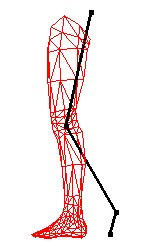
\includegraphics[height=6cm]{../images/fit1}
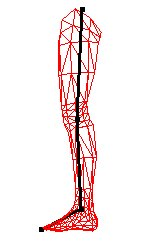
\includegraphics[height=6cm]{../images/fit2}
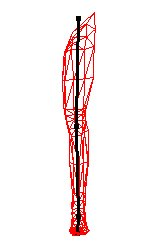
\includegraphics[height=6cm]{../images/fit3}
\caption[Manual Skeleton Fitting]{\label{fig:skeletonfitting} Manual Skeleton Fitting. The skeleton is fitted to the control mesh in two orthogonal views, one joint at a time.}
\end{center}
\end{figure}
The first stage in the process of animating a mesh with a skeleton is to align the two structures correctly, by fitting the skeleton structure to the control mesh. We use a manual interface to individually locate each joint, using two orthogonal viewpoints as shown in figure \ref{fig:skeletonfitting}. This allows the skeleton joint locations to be positioned correctly, ensuring that segment links run through the main structures of the model. The skeleton structure itself is defined manually for each model, but could be constructed interactively with some improvements to the current user interface.

As it is a manual process, the accuracy and repeatability of the skeleton fitting process are limited by the skill of the user. However, in the final system, it is anticipated that this process would be performed by an experienced operator with knowledge of how to position the skeleton model in order to obtain the best results. Incorrectly placed joints will result in unrealistic animation, as joints will appear to rotate around the wrong position.

One possible solution to the repeatability problems would be to generate the skeleton automatically. This would also have the effect of further reducing the manual intervention required in our system. However, no methods for automatic skeleton generation are known of at this time.

\section{\label{sec:skeletalanim:mapping}Control Layer Mapping}

Having located an appropriate skeleton structure inside the mesh we wish to animate, we must now define an automatic mapping between the mesh and the skeleton. Once this mapping is complete, the mesh will be parameterised purely in terms of the skeleton structure, enabling us to drive mesh animation with the skeleton. The mapping must be based purely on the relative locations of skeleton and mesh, as we have no other information available to us, such as higher-level understanding about the two structures. 

We must therefore define a bijective mapping from the space surrounding the skeleton (in which the mesh is embedded) to the skeleton itself. We partition the space into separate regions, each associated with a single segment of the skeleton. Within this region, we then perform a point-to-line mapping to parameterise the mesh vertices in terms of their local segment.

\subsection{\label{sec:skeletalanim:mapping:jointplanes}Joint Planes}
\begin{figure}
\begin{center}
\begin{tabular}{cc}
\setlength{\unitlength}{0.5cm}
\begin{picture}(13,8)
% Joint positions
\put(0,0){\circle*{0.2}}
\put(4,4){\circle*{0.2}}
\put(10,4){\circle*{0.2}}
\put(13,2){\circle*{0.2}}
% Segment links
\put(0,0){\line(1,1){4}}
\put(4,4){\line(1,0){6}}
\put(10,4){\line(3,-2){3}}
% Planes
\put(5,2){\vector(-1,2){2}}
\put(9.33333,2){\vector(1,3){1.3333}}
% Labels
\put(1,0){$\vec{j}_0$}
\put(4.5,4.5){$\vec{j}_1$}
\put(10.5,4.5){$\vec{j}_2$}
\put(13,2.5){$\vec{j}_3$}
\put(3.5,6){$J_1$}
\put(11,6){$J_2$}
\end{picture} &
\setlength{\unitlength}{0.5cm}
\begin{picture}(8,8)
% Joint positions
\put(1,6){\circle*{0.2}}
\put(5,4){\circle*{0.2}}
\put(7,0){\circle*{0.2}}
% Segment links
\thicklines
\put(1,6){\line(2,-1){4}}
\put(5,4){\line(1,-2){2}}
% Joint plane
\thinlines
\put(3,1){\line(0,1){5}}
\put(3,6){\line(2,1){4}}
\put(3,1){\line(2,1){4}}
\put(7,3){\line(0,1){5}}
% Coordinate system
\put(5,4){\vector(0,1){3}}
\put(5,4){\vector(2,1){2}}
\put(5,4){\vector(1,-1){2}}
% Labels
\put(0,6.5){$\vec{j}_{i-1}$}
\put(4,3){$\vec{j}_{i}$}
\put(7.5,0){$\vec{j}_{i+1}$}
\put(7,8){$J_i$}
\put(5.5,6){$\vec{a}_i$}
\put(7.5,5){$\vec{b}_i$}
\put(7.5,2){$\vec{c}_i$}
\end{picture} \\
{\it (a)} & {\it (b)}
\end{tabular}
\caption[Joint Plane Geometry]{\label{fig:jointplanes} Joint Plane Geometry. (a) Joint planes bisect the angles of a skeleton structure. (b) Local coordinate system for a joint plane.}
\end{center}
\end{figure}
We must first partition the space in the region of the skeleton into discrete sections. We do this by defining a {\it joint plane} $J_x\symbol{jointplane}$ for each joint or end effector $\vec{j}_x\symbol{joint}$.

The joint plane $J_x$ is defined as the plane that bisects the joint $\vec{j}_x$, lying equally between the two adjoining segment links, as shown in figure \ref{fig:jointplanes}a. We define $J_x$ using a pair of orthogonal vectors, $\hat{a}_x\symbol{normvector}$ and $\hat{b}_x$. $\hat{a}_x$ is defined as the normal to the plane $P$ defined by the three joint positions $\vec{j}_{x-1}, \vec{j}_x, \vec{j}_{x+1}$, calculated as the normalised cross product of the two adjoining segment vectors.
\begin{eqnarray}
\vec{s}_+ & = & \vec{j}_{x+1} - \vec{j}_x \\
\vec{s}_- & = & \vec{j}_{x-1} - \vec{j}_x \\
\hat{a}_x & = & \frac{\vec{s}_- \times \vec{s}_+}{\|\vec{s}_- \times \vec{s}_+\|}
\end{eqnarray}
$\vec{b}_x$ is defined as the vector that bisects the joint angle, and lies on the plane $P$ as described  above. We calculate this vector as the normalised sum of the two normalised segment vectors:
\begin{eqnarray}
\vec{t} & = & \frac{\vec{s}_-}{\|\vec{s}_-\|} + \frac{\vec{s}_+}{\|\vec{s}_+\|} \nonumber \\
\hat{b}_x & = & \frac{\vec{t}}{\|\vec{t}\|} \label{eqn:jointplaneb}
\end{eqnarray}

Note that $\vec{t}$ is not a new symbol, but simply a temporary vector used to clarify equation \ref{eqn:jointplaneb}. We can also define another useful vector, $\hat{c}_x$, as the cross product of the two vectors $\hat{a}_x$ and $\hat{b}_x$. These three vectors define a local coordinate system, as shown in figure \ref{fig:jointplanes}b.
\begin{equation}
\hat{c}_x = \hat{a}_x \times \hat{b}_x
\end{equation}

\subsubsection{\label{sec:skeletalanim:mapping:jointplanes:special}Special Cases}
There are a number of cases where this formulation is insufficient to define a joint plane. If a joint has multiple child joints, there will be a number of possible values for $\vec{j}_{x+1}$. In this case the average of all these possible values is used for the purposes of plane calculation.

In the case where $\vec{j}_{x-1}$, $\vec{j}_x$ and $\vec{j}_{x+1}$ are colinear, the vector $\vec{a}_x$ is assigned the value of the equivalent vector from the joint plane that lies one level up the skeleton hierarchy, $\vec{a}_{x-1}$. The vector $\vec{b}_x$ is then assigned the value of the normalised cross product $\vec{a}_x \times \vec{s}_-$.

If the joint $\vec{j}_x$ represents an end effector, implying that there is no joint $\vec{j}_{x+1}$ present, $\vec{s}_+$ is assigned the inverted value of $\vec{s}_-$ and the above colinear rule is applied to calculate a valid joint plane.

\subsection{\label{sec:skeletalanim:mapping:pointtoline}Point-To-Line Mapping}

Once we have defined a set of joint planes for a skeleton, we can define a mapping from 3D space onto a single joint segment.  We define the {\it dimensionality} of a segment to be ${\cal S}_n\symbol{segdim}$, where $n$ is one less than the number of bounding planes. We currently only deal with {\it simple} segments, which have only two bounding joint planes, and hence are ${\cal S}_1$. {\it Complex} segments, such as the pelvis, with three or more bounding planes, have a dimensionality of ${\cal S}_n$ where $n>1$, and are discussed below in section \ref{sec:skeletalanim:mapping:complex}.

\begin{figure}
\begin{center}
\setlength{\unitlength}{0.4cm}
\begin{picture}(28,13)
% Points
\put(4,5){\circle*{0.2}}
\put(2,8){\circle*{0.2}}
\put(12,5){\circle*{0.2}}
\put(11,8){\circle*{0.2}}
\put(24,5){\circle*{0.2}}
\put(26,8){\circle*{0.2}}
% Joint planes
\thicklines
\put(1,0){\line(0,1){8}}
\put(1,0){\line(3,1){6}}
\put(7,10){\line(0,-1){8}}
\put(7,10){\line(-3,-1){6}}
\put(21,10){\line(0,-1){8}}
\put(21,10){\line(3,-1){6}}
\put(27,0){\line(0,1){8}}
\put(27,0){\line(-3,1){6}}
% Joint axes
\put(4,5){\vector(0,1){1}}
\put(4,5){\vector(-3,-1){1}}
\put(24,5){\vector(0,1){1}}
\put(24,5){\vector(3,-1){1}}
% Segment links
\put(4,5){\line(1,0){20}}
\thinlines
\put(2,8){\line(1,0){24}}
% Vectors
\put(4,5){\vector(-2,3){2}}
\put(12,5){\vector(-1,3){1}}
\put(24,5){\vector(2,3){2}}
% Labels
\put(6,0){$J_0$}
\put(21,0){$J_1$}
\put(4,4){$\vec{j}_0$}
\put(23,4){$\vec{j}_1$}
\put(1,7){$\vec{p}_0$}
\put(26,7){$\vec{p}_1$}
\put(12,4){$\vec{p}_\alpha$}
\put(11,8.5){$\vec{v}_x$}
\put(6,12.5){$\alpha$}
% Alpha
\put(2,10){\line(0,1){2}}
\put(11,10){\line(0,1){2}}
\put(6,12){\vector(-1,0){4}}
\put(6,12){\vector(1,0){5}}
\end{picture}
\caption[Point To Line Mapping]{\label{fig:pointtoline}Point To Line Mapping}
\end{center}
\end{figure}

The mapping of a 3D point $\vec{v}_x\symbol{vertex}$ onto a line segment is carried out as follows. First of all, $\vec{v}_x$ is projected parallel to the segment, and intersection points $\vec{p}_0\symbol{point}$ and $\vec{p}_1$ calculated with the bounding joint planes, $J_0$ and $J_1$, as shown in figure \ref{fig:pointtoline}.  As the joint planes are infinite in extent, an intersection can always be found, as the planes are never parallel to the projection (segment) vector. 

These intersection points are calculated using standard ray/plane intersection techniques \cite{Lengyel02}. We then calculate a ratio $\alpha_x\symbol{alpha}$, which tells us how far the point $\vec{v}_x$ lies along the segment. The ratio is calculated from the distances between the point $\vec{v}_x$ and the two intersection points.

\begin{equation}
\alpha_x = \frac{\|\vec{v}_x-\vec{p}_0\|}{\|\vec{p}_1-\vec{p}_0\|}
\end{equation}

For instance, a point with $\alpha_x = 0$ would lie on the joint plane $J_0$, while $\alpha_x = 1$ would describe a point lying on the plane $J_1$. A value of 0.5 would define a point lying equidistant between the two planes. The value of $\alpha_x$ describes a plane located between the two bounding joint planes, and which intersects the segment itself at a point $\vec{p}_\alpha$.

\begin{equation} \label{eqn:palpha}
\vec{p}_\alpha = (1 - \alpha_x) \vec{j}_0 + \alpha_x \vec{j}_1
\end{equation}

We then calculate a straight line distance $d_x$ from the point $\vec{p}_\alpha$ to $\vec{v}_x$. 

\begin{equation}
d_x = \|\vec{v}_x - \vec{p}_\alpha\|
\end{equation}

The two parameters $\alpha_x$ and $d_x$ define a circle in 3D space, centred on the point $\vec{p}_\alpha$ and passing through $\vec{v}_x$. In order to uniquely describe the point $\vec{v}_x$, we therefore store a vector $\hat{n}_x$, which is defined as the normal vector to the plane $Q_x$, which passes through $\vec{j}_0$, $\vec{j}_1$ and $\vec{v}_x$. $\vec{p}_0$ and $\vec{p}_1$ also lie on this plane.
\begin{eqnarray}
\vec{t} & = & (\vec{j}_1 - \vec{j}_0) \times (\vec{v}_x - \vec{j}_0) \nonumber \\
\hat{n}_x & = & \frac{\vec{t}}{\|\vec{t}\|}
\end{eqnarray}
Note again that $\vec{t}$ is not a new symbol, but a temporary vector used for clarification. The normal vector $\hat{n}_x$ describes the rotation of the point $\vec{v}_x$ around the segment, and along with the two parameters $\alpha_x$ and $d_x$, uniquely describes the position of the point $\vec{v}_x$. Upon animation, these parameters allow us to deform the 3D position of $\vec{v}_x$ as described below in section \ref{sec:skeletalanim:anim:control}.

\subsection{\label{sec:skeletalanim:mapping:complex}Complex Segments}

The method described above defines a mapping from 3D space onto a line segment. However, complex segments are not represented by a line segment, but by a simplex, the dimensionality of which depends on that of the segment. For instance, an ${\cal S}_2$ segment with three bounding joints would be represented by a triangle, while an ${\cal S}_3$ segment with four bounding joints would be represented by a tetrahedron. The line segment is, of course, the one-dimensional simplex, as is appropriate for an ${\cal S}_1$ segment with two bounding planes. Complex segments are common in skeletal structures; for instance, the human body, while containing mostly ${\cal S}_1$ segments, contains two ${\cal S}_3$ segments at the pelvis and shoulders, and no less than four ${\cal S}_5$ segments, in the hands and feet.

We must therefore generalise our mapping method to map a volume to an $n$-dimensional simplex. The mapping solution defined above works well for ${\cal S}_1$ segments. Additionally, normal-volume mapping, a similar method for mapping points to surfaces described later in section \ref{sec:scandata:pointtosurface}, could be adapted for ${\cal S}_2$ segments. This suggests that it should be possible to formulate a general method of mapping points to ${\cal S}_n$ segments. However, this has not been successful to date, and it is likely that a general mapping solution would be polynomial with degree $n$ or even greater, making the mapping excessively complex even for commonly-occurring segments such as ${\cal S}_5$.

Therefore, we deal only with ${\cal S}_1$ segments from now on, and fix points that lie within complex segments rigidly to that segment, without performing any mapping or deformation.

\subsection{\label{sec:skeletalanim:mapping:mesh}Mesh Mapping}

We define a triangle mesh as a combination of two sets, ${\cal V}\symbol{verts}$ and ${\cal T}\symbol{tris}$. ${\cal V}$ represents the set of vertices in the mesh, and ${\cal T}$ represents the set of triangles, which form the mesh topology.

In order to map a complete mesh to a skeleton, we map each mesh vertex individually. However, we must decide which segment each vertex will map to. In order to calculate this, we must decide which pair of joint planes the vertex lies between. We map each control mesh vertex $\vec{v}_x \in {\cal V}$ to each segment in turn, and calculate its $\alpha_x$ value for that segment. The vertex is assigned to the segment for which the value of $\alpha_x$ lies between 0 and 1, i.e. the vertex $\vec{v}_x$ lies between the joint planes. If this is the case for more than one segment, we calculate the value of $d_x$ for each segment, and assign the vertex to the segment for which it has the lowest value of $d_x$.

\section{\label{sec:skeletalanim:anim}Animation}

Once we have mapped a mesh to the skeleton structure, we can animate that skeleton structure in order to animate the surface of the mesh. This process involves rebuilding the mesh structure from the parameterised representation we have calculated, based on the animated positions of the skeleton's joints.

\subsection{\label{sec:skeletalanim:anim:skeleton}Skeleton Motion}

The animation of the skeleton can be driven by a number of different data sources, from manual keyframed animation, to motion capture systems. In each case however, the data itself is the same. Each frame of animation consists of a set of joint angles which are applied to the joints of the skeleton. The skeleton is then traversed, starting from the root joint and proceeding down the hierarchy, and the cumulative rotation is applied to the default joint positions to position the skeleton into the correct pose. Alternative methods could deliver updated joint positions directly to the skeleton without the use of rotations, but these have the disadvantage that segment lengths are not necessarily preserved, which adversely affects the realism of the animation.

\subsection{\label{sec:skeletalanim:anim:control}Control Layer Deformation}

As the skeleton layer is animated, the joints of the skeleton will change position, which will have the effect of changing the joint planes. As we have parameterised the space around a segment in terms of the joint planes, movement of those planes will deform the parameterised space, and hence the mesh embedded within it. For each animation frame, we need to recalculate a deformed vertex position $\vec{v}_x'$ for each original vertex $\vec{v}_x$. Firstly, the joint planes are updated, by rotating each joint plane by half of the rotation of its associated joint. This ensures that the joint plane still bisects the joint angle.

For each vertex $\vec{v}_x \in {\cal V}$, we can calculate a deformed vertex position $\vec{v}_x'$ using the stored parameters $\alpha_x$, $d_x$, and $\hat{n}_x$. We start by calculating a pair of vectors $\hat{s}_0$ and $\hat{s}_1$ on the bounding planes. These vectors define the direction in which the deformed points $\vec{p}_0$ and $\vec{p}_1$ lie on the rotated joint planes.
\begin{eqnarray} \label{eqn:normals}
\hat{s}_0 & = & \hat{c}_0 \times \hat{n}_x \\ 
\hat{s}_1 & = & \hat{c}_1 \times \hat{n}_x
\end{eqnarray}
We then calculate a vector $\vec{s}_\alpha$ as a linear interpolation of $\hat{s}_0$ and $\hat{s}_1$, as well as a point $\vec{p}_\alpha$ on the line segment. This tells us the point on the segment that the original $\vec{v}_x$ mapped to, and the direction in which the deformed $\vec{v}_x'$ should lie.
\begin{eqnarray}
\vec{s}_\alpha & = & (1 - \alpha_x) \hat{s}_0 + \alpha_x \hat{s}_1 \\
\vec{p}_\alpha & = & (1 - \alpha_x) \vec{j}_0' + \alpha_x \vec{j}_1' 
\end{eqnarray}
We then calculate the new vertex position $\vec{v}_x'$ by multiplying the $\vec{s}_\alpha$ by the stored distance value $d_x$, and adding to $\vec{p}_\alpha$.
\begin{equation}
\vec{v}_x' = \vec{p}_\alpha + d_x \vec{s}_\alpha
\end{equation}
\begin{figure}
\begin{center}
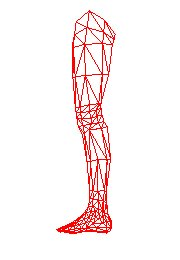
\includegraphics[width=3.18cm]{../images/low_leg_1}
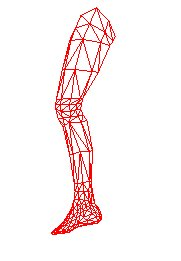
\includegraphics[width=3.18cm]{../images/low_leg_2}
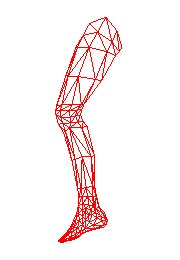
\includegraphics[width=3.18cm]{../images/low_leg_3}
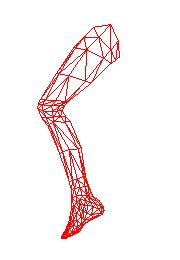
\includegraphics[width=3.18cm]{../images/low_leg_4}
\caption[Control Mesh Animation]{\label{fig:controlmesh} Control Mesh Animation.}
\end{center}
\end{figure}
This formulation gives an efficient deformation for each point, well suited for realtime calculation. Figure \ref{fig:controlmesh} illustrates the skeletal animation of a simple mesh, showing how the shape of the mesh deforms as the skeleton bends.

\subsection{\label{sec:skeletalanim:anim:collapse}Segment Collapse}

The above method works well for small changes in the pose of the skeleton, but large angles at joints can introduce errors. The linear interpolation of the plane vectors introduces thinning effects near joints, orthogonal to the axis of the joint rotation. Also caused by this is the complete collapse of segments under twisting rotations. Both of these effects are highly undesirable.

A method of avoiding these problems was described by Wei Sun in \cite{Sun01}. This method compensates for the thinning effects by introducing a term into the reconstruction equations that causes a reconstructed point to maintain a fixed distance from the nearest point on the segment, or from a joint centre if that is closer. This method prevents the thinning of the surface, as well as sharp creases near joints, giving a smooth deformation of the mesh surface.

\section{\label{sec:skeletalanim:vrml}VRML Implementation}
\nomenclature{\bf VRML}{The Virtual Reality Modelling Language, a programming language for describing 3D scenes and objects.}
In order to demonstrate the efficiency of the skeletal animation method described above, we have created an implementation of the algorithm in the VRML97 3D modelling language \cite{VRML97}. In order to do this, we also describe a novel method for the animation of deformable models in VRML, which we originally introduced in \cite{Smith00}.

\subsection{\label{sec:skeletalanim:vrml:hanim}H-Anim Compliant Humans}

We base our method on the existing H-Anim 1.1 specification \cite{HANIM99} for the animation of articulated characters in VRML. The H-Anim standard defines a set of VRML extensions which are used to represent articulated models, in particular humanoid figures. These extensions are implemented using the PROTO mechanism, which allows new VRML nodes to be defined in terms of the standard set of nodes \footnote{In the following description, names of VRML nodes are written in {\bf bold} type, while field and other names are written in {\it italics}.}

H-Anim defines a number of new VRML nodes; firstly, it defines the {\bf Humanoid} node, which acts as a container for an articulated model structure. This node contains within it a hierarchy of {\bf Joint} nodes, which form the skeleton structure itself. The skeleton is posed by assigning rotation values to each of these joint nodes. Each {\bf Joint} has a name associated with it, assigned by a special naming scheme. For instance, the left shoulder joint is named {\it l\_shoulder}. A single joint forms the root of the hierarchy, named {\it HumanoidRoot}. 

The joints define the articulation structure of the model, but the geometry of the body is defined inside {\bf Segment} nodes. Each {\bf Joint} contains a single {\bf Segment}, corresponding to the part of the body directly affected by that joint and named accordingly. For instance, the {\it l\_shoulder} joint will have a child segment named {\it l\_upperarm}. {\bf Segment}s contain geometry information for that section of the model, so the {\it l\_upperarm} will typically contain an {\bf IndexedFaceSet} node containing a rigid 3D model for the upper arm.

A {\bf Segment} node can also contain any number of {\bf Site} nodes. These nodes store single 3D points, for use as end effectors, or attachment points for clothing and accessories. If we consider a segment representing the left hand, {\it l\_hand}, it will contain a site representing an end effector, named {\it l\_hand\_tip}.

\subsection{\label{sec:skeletalanim:vrml:extentions}Extending H-Anim for Seamless Models}
As VRML97 does not allow non-rigid transformations of objects, it is impossible to represent deformable seamless\footnote{A seamless surface will be C0 continuous, i.e. will not contain any cracks.} models using pure VRML. However, the VRML97 {\bf Script} node allows a programmer to add functionality to the language by using Java \cite{Gosling00} or ECMAScript \cite{ECMA99} to write code that can be executed as part of a VRML scene. We can implement the mesh deformation algorithm using this facility, but we must first define a VRML structure which will represent the seamless model. We base our structure around H-Anim 1.1, but add a number of new elements. We take a different approach to previous methods \cite{Babski99}, and define the surface as a single polygon mesh, while separating geometric and topological properties.

First, we calculate which segment each vertex should be assigned to, using the method described in section \ref{sec:skeletalanim:mapping:mesh}. The vertices are then re-ordered so that they are arranged in contiguous sets of vertices that are assigned to the same segment. The set of vertices for each segment is then stored in the {\it coord} field of the appropriate {\bf Segment} node.

We then define a new node, {\bf MeshBody}  (see figure \ref{fig:meshbodyproto}), to store the remaining mesh data including topology, texture and colour information. This node is implemented as a combination of an {\bf IndexedFaceSet} and a {\bf Script} node. The mesh data is stored in the {\bf IndexedFaceSet} part, and the {\bf Script} contains a Java or ECMAScript implementation of the deformation engine. The {\bf MeshBody} node itself is stored inside a new field which we add to the {\bf Humanoid} node, called {\it meshBody}. The extended {\bf Humanoid} node is shown in figure \ref{fig:humanoidproto}.

\begin{figure}
\renewcommand{\baselinestretch}{1}
\scriptsize
\begin{verbatim}
PROTO MeshBody [
 exposedField SFString   name             ""
 exposedField MFString   info             []
 exposedField SFNode     appearance       NULL
 exposedField SFNode     color            NULL
 exposedField SFNode     normal           NULL
 exposedField SFNode     texCoord         NULL     
 field        SFBool     ccw              TRUE
 field        MFInt32    colorIndex       []
 field        SFBool     colorPerVertex	  TRUE
 field        SFBool     convex           TRUE
 field        MFInt32    coordIndex       []
 field        SFFloat    creaseAngle      0
 field        MFInt32    normalIndex      []
 field        SFBool     normalPerVertex  TRUE
 field        SFBool     solid            TRUE
 field        MFInt32    texCoordIndex    []
 field        SFBool     mustEvaluate     FALSE
 field        SFNode     humanoid         NULL
 field        MFString   url              []
 eventIn      SFTime     update
]
{
  Group {
    children [
      Shape {
        appearance IS appearance
        geometry IndexedFaceSet {
          color IS color
          normal IS normal
          texCoord IS texCoord
          ccw IS ccw
          colorIndex IS colorIndex
          colorPerVertex IS colorPerVertex
          convex IS convex
          coordIndex IS coordIndex
          coord DEF BODYCOORDS Coordinate {}
          creaseAngle IS creaseAngle
          normalIndex IS normalIndex
          normalPerVertex IS normalPerVertex
          solid IS solid
          texCoordIndex IS texCoordIndex
        }
      }
      DEF SEAMLESSBODY Script {
        url IS url
        directOutput TRUE
        mustEvaluate IS mustEvaluate
        field SFNode humanoid IS humanoid
        field SFNode bodyCoords USE BODYCOORDS
        eventIn SFTime update IS update
      }
    ]
  }
}
\end{verbatim}
\caption[The MeshBody Prototype]{\label{fig:meshbodyproto} The {\bf MeshBody} Prototype. The new node is basically a fusion of an {\bf IndexedFaceSet} and a {\bf Script}.}
\end{figure}

\begin{figure}[t]
\renewcommand{\baselinestretch}{1}
\scriptsize
\begin{verbatim}
PROTO Humanoid [
 exposedField SFVec3f    center           0 0 0
 exposedField MFNode     humanoidBody     [ ]
 exposedField MFString   info             [ ]
 exposedField MFNode     joints           [ ]
 exposedField SFNode     meshBody         NULL              # NEW
 exposedField SFString   name             ""
 exposedField SFRotation rotation         0 0 1 0
 exposedField SFVec3f    scale            1 1 1
 exposedField SFRotation scaleOrientation 0 0 1 0
 exposedField MFNode     segments         [ ]
 exposedField MFNode     sites            [ ]
 exposedField SFVec3f    translation      0 0 0
 exposedField SFString   version          "1.1"
 exposedField MFNode     viewpoints       [ ]
]
{
  Transform {
    center IS center
    rotation IS rotation
    scale IS scale
    scaleOrientation IS scaleOrientation
    translation IS translation
    children [
      Group {
        children IS viewpoints
      }
      Group {
        children IS humanoidBody
      }
      Group {                                               # NEW
        children IS meshBody                                # NEW
      }                                                     # NEW
    ]
  }
}
\end{verbatim}
\caption[The Extended Humanoid Prototype.]{\label{fig:humanoidproto} The Extended {\bf Humanoid} Prototype. Our extensions are marked with comments.}
\end{figure}

\subsection{\label{sec:skeletalanim:vrml:animation}Animation}
During a single frame of animation, a set of rotations are applied to the joints in the structure, posing the skeleton. The Java code inside the {\bf Script} node then traverses the hierarchy, deforming the vertices contained in the {\it coord} field of each {\bf Segment} appropriately, and merging them into a single vertex list which is placed into the {\bf IndexedFaceSet} section of the {\bf MeshBody} node, in order to set the geometry of the mesh for display. This method deforms the mesh seamlessly by modifying the vertices of a single mesh separately.

\subsection{\label{sec:skeletalanim:vrml:engine}The Deformation Engine}

The actual deformation process is performed wholly within a Java program stored in the {\bf Script} section of the {\bf MeshBody} node. The internal structure of the script consists of an {\it init} function, which is called when the model is loaded, and an {\it eventsProcessed} function which is called once per frame.

The {\it init} method traverses the skeleton hierarchy, calculating joint planes and performing the mapping process described in section \ref{sec:skeletalanim:mapping}. The joint planes and mapped vertices are cached inside the script for later reconstruction. 

\begin{figure}
\begin{center}
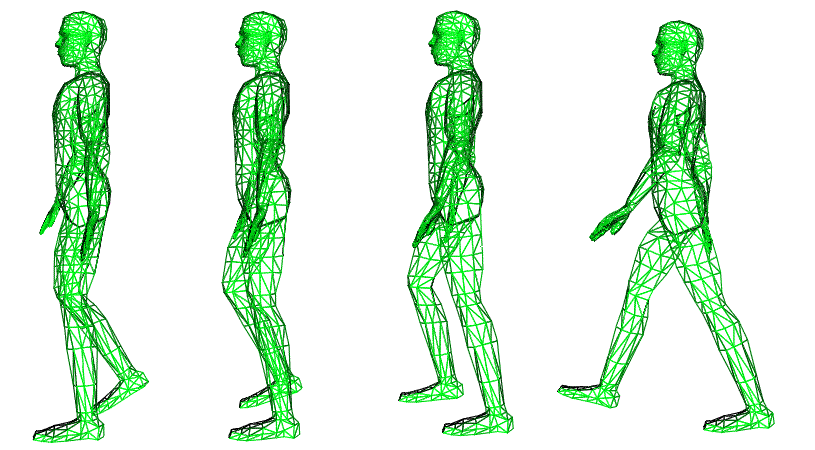
\includegraphics[width=14cm]{../images/simpleanimation}
\caption[Seamless VRML Humans]{\label{fig:simplesegments} Seamless VRML Humans. This figure shows our skeletal animation technique, applied to a human body model in VRML. }
\end{center}
\end{figure}

The {\it eventsProcessed} method is then called before each frame is displayed on screen. This method traverses the skeleton hierarchy again, reading the joint rotations and updating its internal cache of joint planes. The reconstruction process described in section \ref{sec:skeletalanim:anim} is then carried out for each vertex. The vertices are fused into a single list, and output into the {\it bodyCoords} field of the {\bf Script}, which is in turn a reference to the {\it coord} field of the {\bf IndexedFaceSet}. The VRML browser then displays the deformed mesh, an example of which is shown in figure \ref{fig:simplesegments}.

The VRML structures only define the interface to the deformation engine script, not its behaviour. Therefore,  any deformation scheme could be used in conjunction with this structure, not necessarily the one we describe above. The deformation engine must simply read rotations from the hierarchy, read coordinates from the segments, and output a  set of deformed coordinates into its {\it bodyCoords} field each frame. The deformation engine can be treated as a `black box' system.

\subsection{\label{sec:skeletalanim:vrml:hanim2001}H-Anim 2001}

Since this method was introduced, elements of the design have been integrated into the H-Anim 2001 specification \cite{HANIM2001}. This latest version of the specification adds support for seamless deformable models, using a technique based in part on that presented above. The {\bf Humanoid} stores a single list of coordinates, which are referenced by a set of {\bf IndexedFaceSet} nodes which form the surface of the seamless object. Each {\bf Segment} then contains a list of indices of coordinates that are affected by that segment, as well as a set of weights for those vertices. The {\bf Humanoid} node also contains a script, which implements a deformation engine. The specification is designed to include a generic vertex blending deformation engine, but there is no reason why a different animation algorithm could not be used instead.

\section{\label{sec:skeletalanim:results}Results}

\begin{figure}
\begin{center}
\begin{tabular}{ccc}
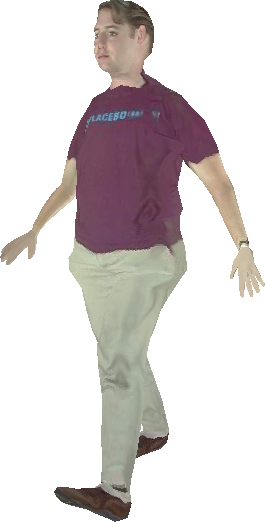
\includegraphics[height=5cm]{../images/james_texture1} &
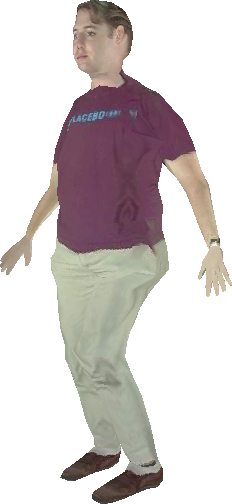
\includegraphics[height=5cm]{../images/james_texture2} &
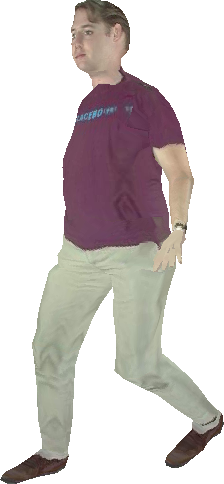
\includegraphics[height=5cm]{../images/james_texture3} \\
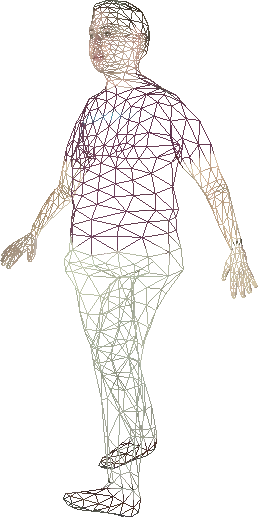
\includegraphics[height=5cm]{../images/james_wire1} &
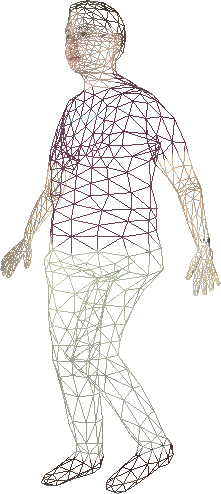
\includegraphics[height=5cm]{../images/james_wire2} &
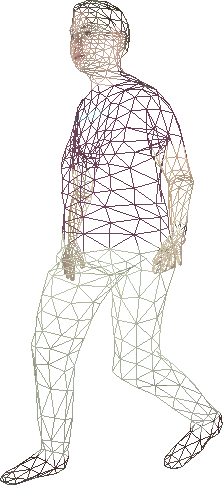
\includegraphics[height=5cm]{../images/james_wire3} \\
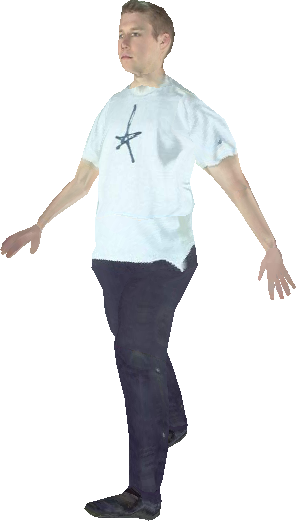
\includegraphics[height=5cm]{../images/warren_texture1} &
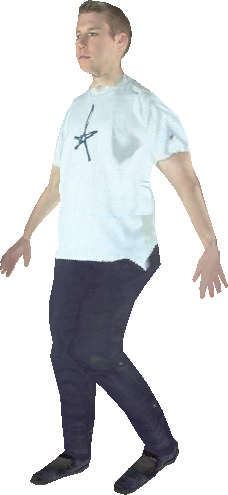
\includegraphics[height=5cm]{../images/warren_texture2} &
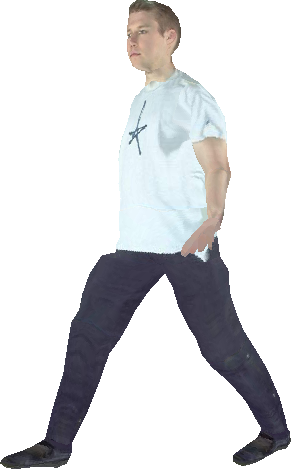
\includegraphics[height=5cm]{../images/warren_texture3} \\
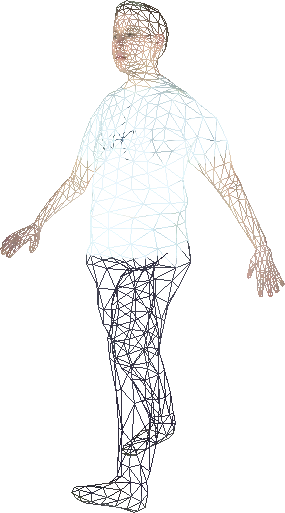
\includegraphics[height=5cm]{../images/warren_wire1} &
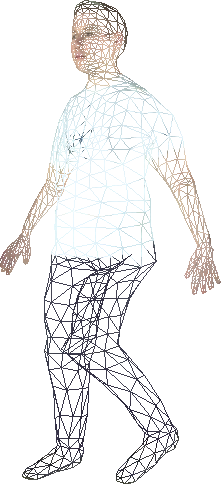
\includegraphics[height=5cm]{../images/warren_wire2} &
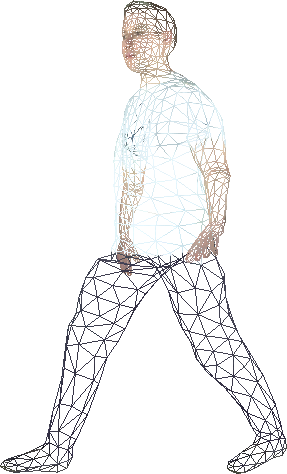
\includegraphics[height=5cm]{../images/warren_wire3} \\
\end{tabular}
\caption[Control Mesh Animation]{\label{fig:controlanim} Control Mesh Animation, showing animation of two human models in VRML, using our deformation technique. The models were generated using the AvatarBooth body scanner from \citet{AvatarMe}.}
\end{center}
\end{figure}

Figure \ref{fig:controlanim} shows our skeletal animation technique applied to a pair of human body models. These models were animated in real time using the VRML implementation of our deformation engine. Surface discontinuities can be seen in places, as the implementation only deals with ${\cal S}_1$ segments, as discussed earlier. Complex segments such as the pelvis are transformed rigidly with their parent joint.

\section{\label{sec:skeletalanim:conclusion}Conclusion}

We have presented a novel method of performing skeletal animation, which uses a fully-automatic mapping process to perform deformations of the surface based on a manually positioned skeleton structure. The algorithm is efficient, able to execute in real time even when run inside an interpreted VRML script. However, the algorithm cannot currently support deformation of complex body segments, as no method has yet been developed to extend the automatic mapping process to higher dimensions.

We have also presented a novel method of defining seamless deformable objects in VRML97, which has since been integrated in part into the H-Anim 2001 specification, which is intended for ISO standardisation.

Our skeletal animation method allows an animator to animate a low-resolution mesh in real time, by manipulating the skeleton structure. The next stage in our layered animation method is to apply the animation of this low resolution mesh to the dense scanned data that we actually wish to deform. This should enable accurate translation of the low resolution animation to a highly detailed surface.

\subsection{\label{sec:skeletalanim:conclusion:future}Future Work}

The skeletal animation method presented in this chapter can be improved in a number of ways. Firstly, as discussed in section \ref{sec:skeletalanim:mapping:complex}, we can currently only cope with simple segments with two bounding joints. This is insufficient to animate complex models effectively, and so the method should be extended to support animation of complex segments. Additionally, it may be useful to use a higher order function to interpolate along each segment, rather than a simple linear interpolation. This has not been investigated however, and would need further research, but has the potential to create mathematically smooth animation of the surface.

During development of the linear interpolation method described above, another method was proposed which has not been implemented, but which is worthy of further research. Instead of using a linear interpolation of end plane points, we propose a method of performing skeletal animation using quaternion-based interpolation. The $\alpha_x$ coordinate of a point would still be calculated as above, but instead of calculating $d_x$ and $\hat{n}_x$, we simply store $\vec{q}_x$, which is a vector from the point $\vec{p}_\alpha$ to $\vec{v}_x$. Each frame, a rotation is calculated that rotates $J_0$ onto $J_1$, and this rotation is interpolated along the segment using spherical linear interpolation of quaternions \cite{Lengyel02}. The interpolated rotation is applied to each vector $\vec{q}_x$ to create a deformed version of each point. This method should reduce collapse due to twisting, giving a more robust animation of the control layer. 
